\documentclass[10pt,xcolor={dvipsnames}]{beamer}

\mode<presentation>{
  \usetheme{CambridgeUS}
  \usecolortheme{sysnove}
  \setbeamercovered{transparent}
}

%\usepackage[french]{babel}
\usepackage[utf8]{inputenc}
\usepackage{default}

\usepackage{ifthen}
\usepackage{listings}
\usepackage{tcolorbox}
\tcbuselibrary{listings, raster, xparse}
\usepackage{tikz}
\usetikzlibrary{calc, tikzmark}

\graphicspath{{imgs/}}

\title[Outils de travail collaboratif]{{\small ADSILLH}\\Outils de travail collaboratif}
\author[Alexis Lahouze]{Alexis~\textsc{Lahouze}\\
  \medskip
  
\includegraphics[scale=0.5]{logo-sysnove}
}
\institute[Sysnove]{}
\date{ADSILLH 2016 S1}

\setbeamerfont{author in sidebar}{size=\footnotesize}
\setbeamerfont{title in sidebar}{size=\footnotesize}
\setbeamerfont{subsection in sidebar}{size=\scriptsize}
\setbeamercolor{palette sidebar secondary}{fg=darkred}
\setbeamercolor{title in sidebar}{fg=darkred}

\setbeamertemplate{navigation symbols}{}

\logo{
  
\includegraphics[height=0.6cm]{logo-sysnove}
  \hspace{0.5cm}
}

\usepackage{nameref}
\makeatletter
\newcommand*{\currentname}{\@currentlabelname}
\makeatother

\AtBeginSection[]
{
  \begin{frame}{\currentname}
    \tableofcontents[
      currentsection,
      sectionstyle=show/shaded,
      subsectionstyle=show/show/hide
    ]
  \end{frame}
}

% Define listings global style
\lstset{
  %frame=single,
  %breaklines=true,
  basicstyle=\ttfamily\tiny,
  numberstyle=\ttfamily\tiny,
  numbersep=5pt,
  %postbreak=\raisebox{0ex}[0ex][0ex]{\ensuremath{\color{red}\hookrightarrow\space}}
  escapeinside=||
}

% Define diff language for listings
\lstdefinelanguage[normal]{diff}{
  morecomment=[f][\color{BrickRed}]<,         % deleted lines 
  morecomment=[f][\color{ForestGreen}]>,      % added lines
}


\NewTCBListing{snvlisting}{ O{} m }{%
  colback=red0!10!white,
  colframe=red0!75!black,
  title=#2 (#1),
  fonttitle=\tiny,
  lowerbox=ignored,
  listing only,
  listing options={%
    basicstyle=\tiny\ttfamily,
    numberstyle=\tiny\ttfamily,
    numbers=left,
    escapeinside=||,
    language={#1}}}%

% Command to draw a balloon over two anchors
%\newcommand<>{\balloon}[3]{%
%  \coordinate (c) at ($(#2)+(0,1ex)$);
%  \node#4 (#1) [balloon, fit=(#3) (c)] {};}

\begin{document}
\begin{frame}[plain]
  \titlepage
\end{frame}

\begin{frame}[squeeze]{Sommaire}
  \tableofcontents[sectionstyle=show, subsectionstyle=show/show/show]
\end{frame}

\section{Développement}
\subsection{Patch}

\begin{frame}{Premiers patchs}
 \begin{figure}
   \caption{Programme sur bande perforée patchée pour Harvard Mark I.}
   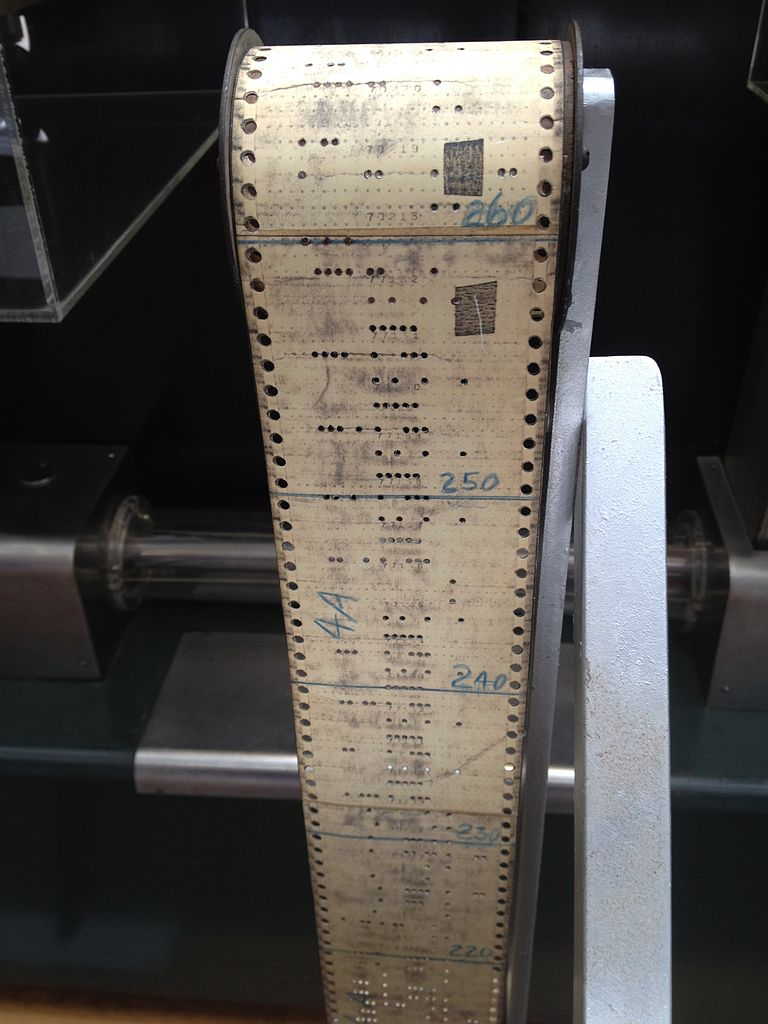
\includegraphics[height=160pt]{Harvard_Mark_I_program_tape}\par
   \tiny Source~: Wikipedia
 \end{figure}
\end{frame}

\begin{frame}[fragile]{Principe de base}
Sortie normale de diff

\begin{tcbraster}[raster columns=3, raster valign=top]
      \begin{snvlisting}{Original}
This part of the
document has stayed the
same from version to
version.  It shouldn't
be shown if it doesn't
change.  Otherwise, that
would not be helping to
compress the size of the
changes.
      \end{snvlisting}
      \begin{snvlisting}{Modifié}
This is an important
notice! It should
therefore be located at
the beginning of this
document!
      \end{snvlisting}
      \begin{tcolorbox}[blanker]
      \begin{tcbraster}[raster columns=1, raster rows=2]
      \begin{snvlisting}[[normal]diff]{Diff}
|\tikzmark{b}|0a1,6|\tikzmark{c}|
> This is an important
> notice! It should
> therefore be located at
> the beginning of this
> document!
      \end{snvlisting}
      \
      \end{tcbraster}
      \end{tcolorbox}
\end{tcbraster}
\begin{tikzpicture}[overlay,remember picture]
  \draw ([yshift=5pt]pic cs:b) rectangle ([yshift=-2pt]pic cs:c);
\end{tikzpicture}
\end{frame}

\end{document}

